%!TEX root = ../thesis.tex
%*******************************************************************************
%****************************** Second Chapter *********************************
%*******************************************************************************
\graphicspath{{Chapter2/Figs/Vector/}{Chapter2/Figs/}}

%%%%%%%%%%%%%%%%%%%%%%%%%%%%%%%%%%%%%%%%%%%%%%%%%%%%%%%%%%%%%%%%%%%%%%%%%%%%%%%%
% Encoding Locations
%%%%%%%%%%%%%%%%%%%%%%%%%%%%%%%%%%%%%%%%%%%%%%%%%%%%%%%%%%%%%%%%%%%%%%%%%%%%%%%%
% - In what way can locations be represented to be universally interpretable
%   and precise?
%
\chapter{Encoding Locations}
\section{Introduction}
Encoding of locations has historically been of great importance, and is always being modernized. This chapter explains the general definition of locations, which types of locations are important for this project, and how to represent these locations so that they are universally interpretable and do not rely on a postal code system.

%%%%%%%%%%%%%%%%%%%%%%%%%%%%%%%%%%%%%%%%%%%%%%%%%%%%%%%%%%%%%%%%%%%%%%%%%%%%%%%%
% A Brief History Of Geographic Locations
%%%%%%%%%%%%%%%%%%%%%%%%%%%%%%%%%%%%%%%%%%%%%%%%%%%%%%%%%%%%%%%%%%%%%%%%%%%%%%%%
% - How did the history of navigation evolve?
% - Who and what played a big role in navigation?
%
\section{A Brief History Of Geographic Locations}
A location is roughly described as a place or position. Throughout history, various navigational techniques and tools like the sextant, nautical chart and marinner's compass were used, measuring the altitude of the North Star to determine the latitude $\phi$, in conjunction with a chronometer to determine the longitude $\lambda$ of a location on the Earth's surface. The combination of coordinates is a distinct encoding of a location. This particular system is still commonly used today.

\begin{figure}[htbp!]
	\centering
	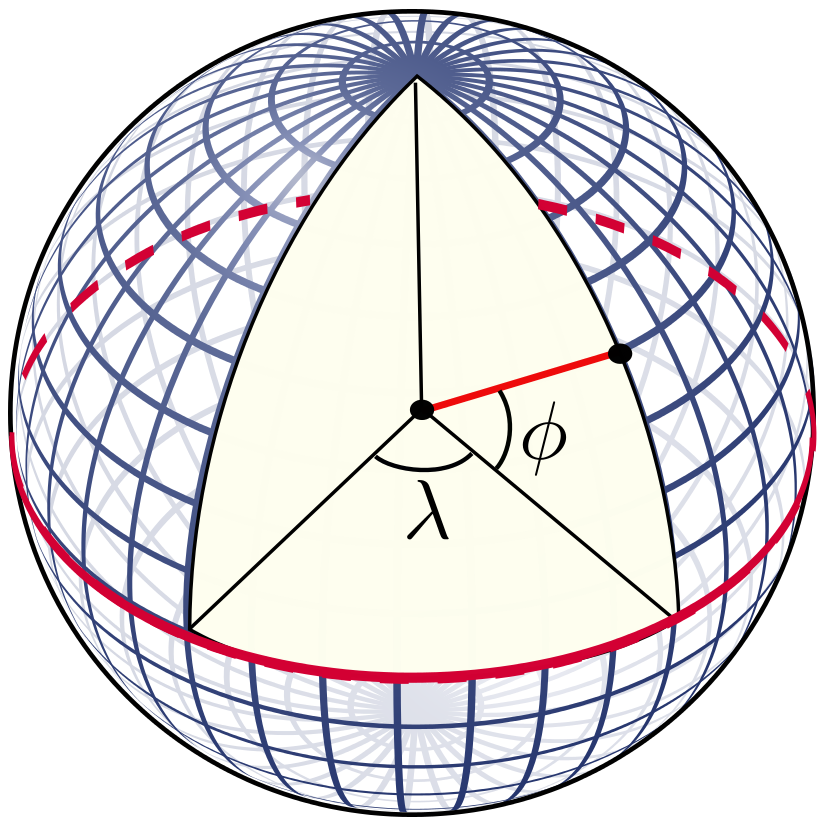
\includegraphics[width=.2\textwidth]{LatLngSphere}
	\caption[LatLngSphere]{A perspective view of the Earth showing how latitude and longitude are defined on a spherical model.}
	\label{fig:latlngsphere}
\end{figure}

The history of this encoding goes way back to when it was first proposed in the 3rd century BC by Eratosthenes. He invented the discipline of geography, and was known for also being the first person to calculate the circumference of the Earth with remarkable accuracy. Today, navigation relies on satellites that are capable of providing information to determine a location with a precision of 9 meters. Hybrid methods using cell towers, Wi-Fi Location Services, and the new Galileo global navigation sattelite system, provide tracking with a precision down to the metre range. These locations are ordinarily communicated using the same established latitude and longitude encoding. For a human being, it is not practical to exchange day-to-day locations as geographical coordinates. For that, addresses much more suitable, but can be ambiguous, imprecise, and inconsistent in format. Addresses commonly make use of Postal Code systems, which have reliably been assigned to geographical areas with the purpose of sorting mail. Although even today, there are countries that do not have a Postal Code system. This forces the legacy system to support addresses for the fixed pricing functionality as well. In contrast to the geographic coordinate system, postal codes describe streets and areas of varying shapes and sizes. A location being roughly described as a place or position, can be decomposed as an abstract term to describe physical or imaginary areas with varying radiusses and shapes. You could prepend 'the location of' to the following terms as an example: America, the birthplace of Sokrates, Wall Street, the center of the universe, the Laryngeal Nerve of the Giraffe, churches in the Netherlands. The final example presents the main challenge of this project, how to communicate the location of a collection with points or areas of differing shapes and sizes that may overlap?

%%%%%%%%%%%%%%%%%%%%%%%%%%%%%%%%%%%%%%%%%%%%%%%%%%%%%%%%%%%%%%%%%%%%%%%%%%%%%%%%
% Requisites of Location types
%%%%%%%%%%%%%%%%%%%%%%%%%%%%%%%%%%%%%%%%%%%%%%%%%%%%%%%%%%%%%%%%%%%%%%%%%%%%%%%%
% - What do we need to describe our type of locations?
% - What do we not need?
% - Which location types matter for this project?
% - What are the main differences between postal systems used around the globe?
% - Can postal codes be abstracted to geospatial data while retaining the same
%   usefulness in the system?
%
\section{Requisites of Location Types}
While setting up a backlog for a project, a shared knowledge about the terminology used in the issues must be achieved in order to collaborate effectively. Words or symbols do not have an absolute meaning, and ambiguity of abstract linguistic terms should be elucidated. In section 3.2.1 of Appendix \ref{appendix:pregame}, an agreement was made on what the terms "area" and "point" meant. During the process of implementing TPS, the definitions of a location have been refined.

\subsection{The Point}
A point is a unique place expressed as a distinct coordinate pair. An address in the legacy system could be translated to a point. For example, the address that is tied to Schiphol arrival is: Aankomstpassage, 1118 AX Schiphol Centrum.
The point that encodes this location is (52.308891, 4.760900). This location is contained in the set of all possible points on Earth, which could be expressed using set builder notation:
\[P = \{(\phi,\lambda) \in \mathbb{R}^2 | -90 < \phi < 90, -180 < \lambda < 180 \}\]
\[(52.308891, 4.760900) \in P\]
A point itself can not be used to match whether another point is contained within it, because the probability of a match is infitesimal. Only when decimals were disregarded to decrease the precision of a point it would be possible, in which case it would still not be usefull in this application, because the imprecise point would be a square.

\subsection{The Area}
An area is a set of three or more points that is tightly packed together with an infinite granularity. This definition allows for an area to have holes inside them, consist of other locations and contain other locations, and be infinitely precise. The most useful property of this area is to check whether a point is contained within the area, or which areas contain a given point. A line, which could be constructed with this definition, would essentially be useless for containment matching for the same reasons as a point would be useless. This definition, however conceptually valuable, will not be of much practical use. For example, $P$ is an infinitely long set of coordinates, an area that represents the earths surface. If $\phi$ ranged between 0 and 90, the set sould describe all points located in the northern hemisphere, but would still be infinitely long. So, an area can be described as a subset of all points:
\[A \subseteq P \]
At the equator, 1 degree is 111320m, so 0.000001 degrees is
around 11cm. Six decimal places will be sufficient for location matching for this application. Checking whether a given point is contained by checking an infinite amount of real number pairs will take an infinite amount of time in the worst case scenario, but even when reducing coordinates to having six decimal places, it would be impractical. For this reason, it is more realistic to only describe the edges of an area using a polygon shape. For example: all postal codes of the city of Amsterdam start with a ten, the entire area of Amsterdam can be drawn as a big polygon containing all the postal codes that start with a ten.

\subsection{United Arab Emirates}
In reverse, this procedure would not work. Postal codes are not flexible or precise enough to describe area's the way polygons would. If a client wanted to convert a polygon containing two halves of neighbouring provinces to a postal code, it would be impossible. One big taxi company that makes use of taxiID's legacy system located in the United Arab Emirates would not be able to convert anything at all, beause the United Arab Emirates does not have a postal code system to begin with. When a trip is booked in the United Arab Emirates, the only information provided as a destination or departure location are geospatial coordinates and addresses.

\begin{figure}[htbp!]
	\centering
	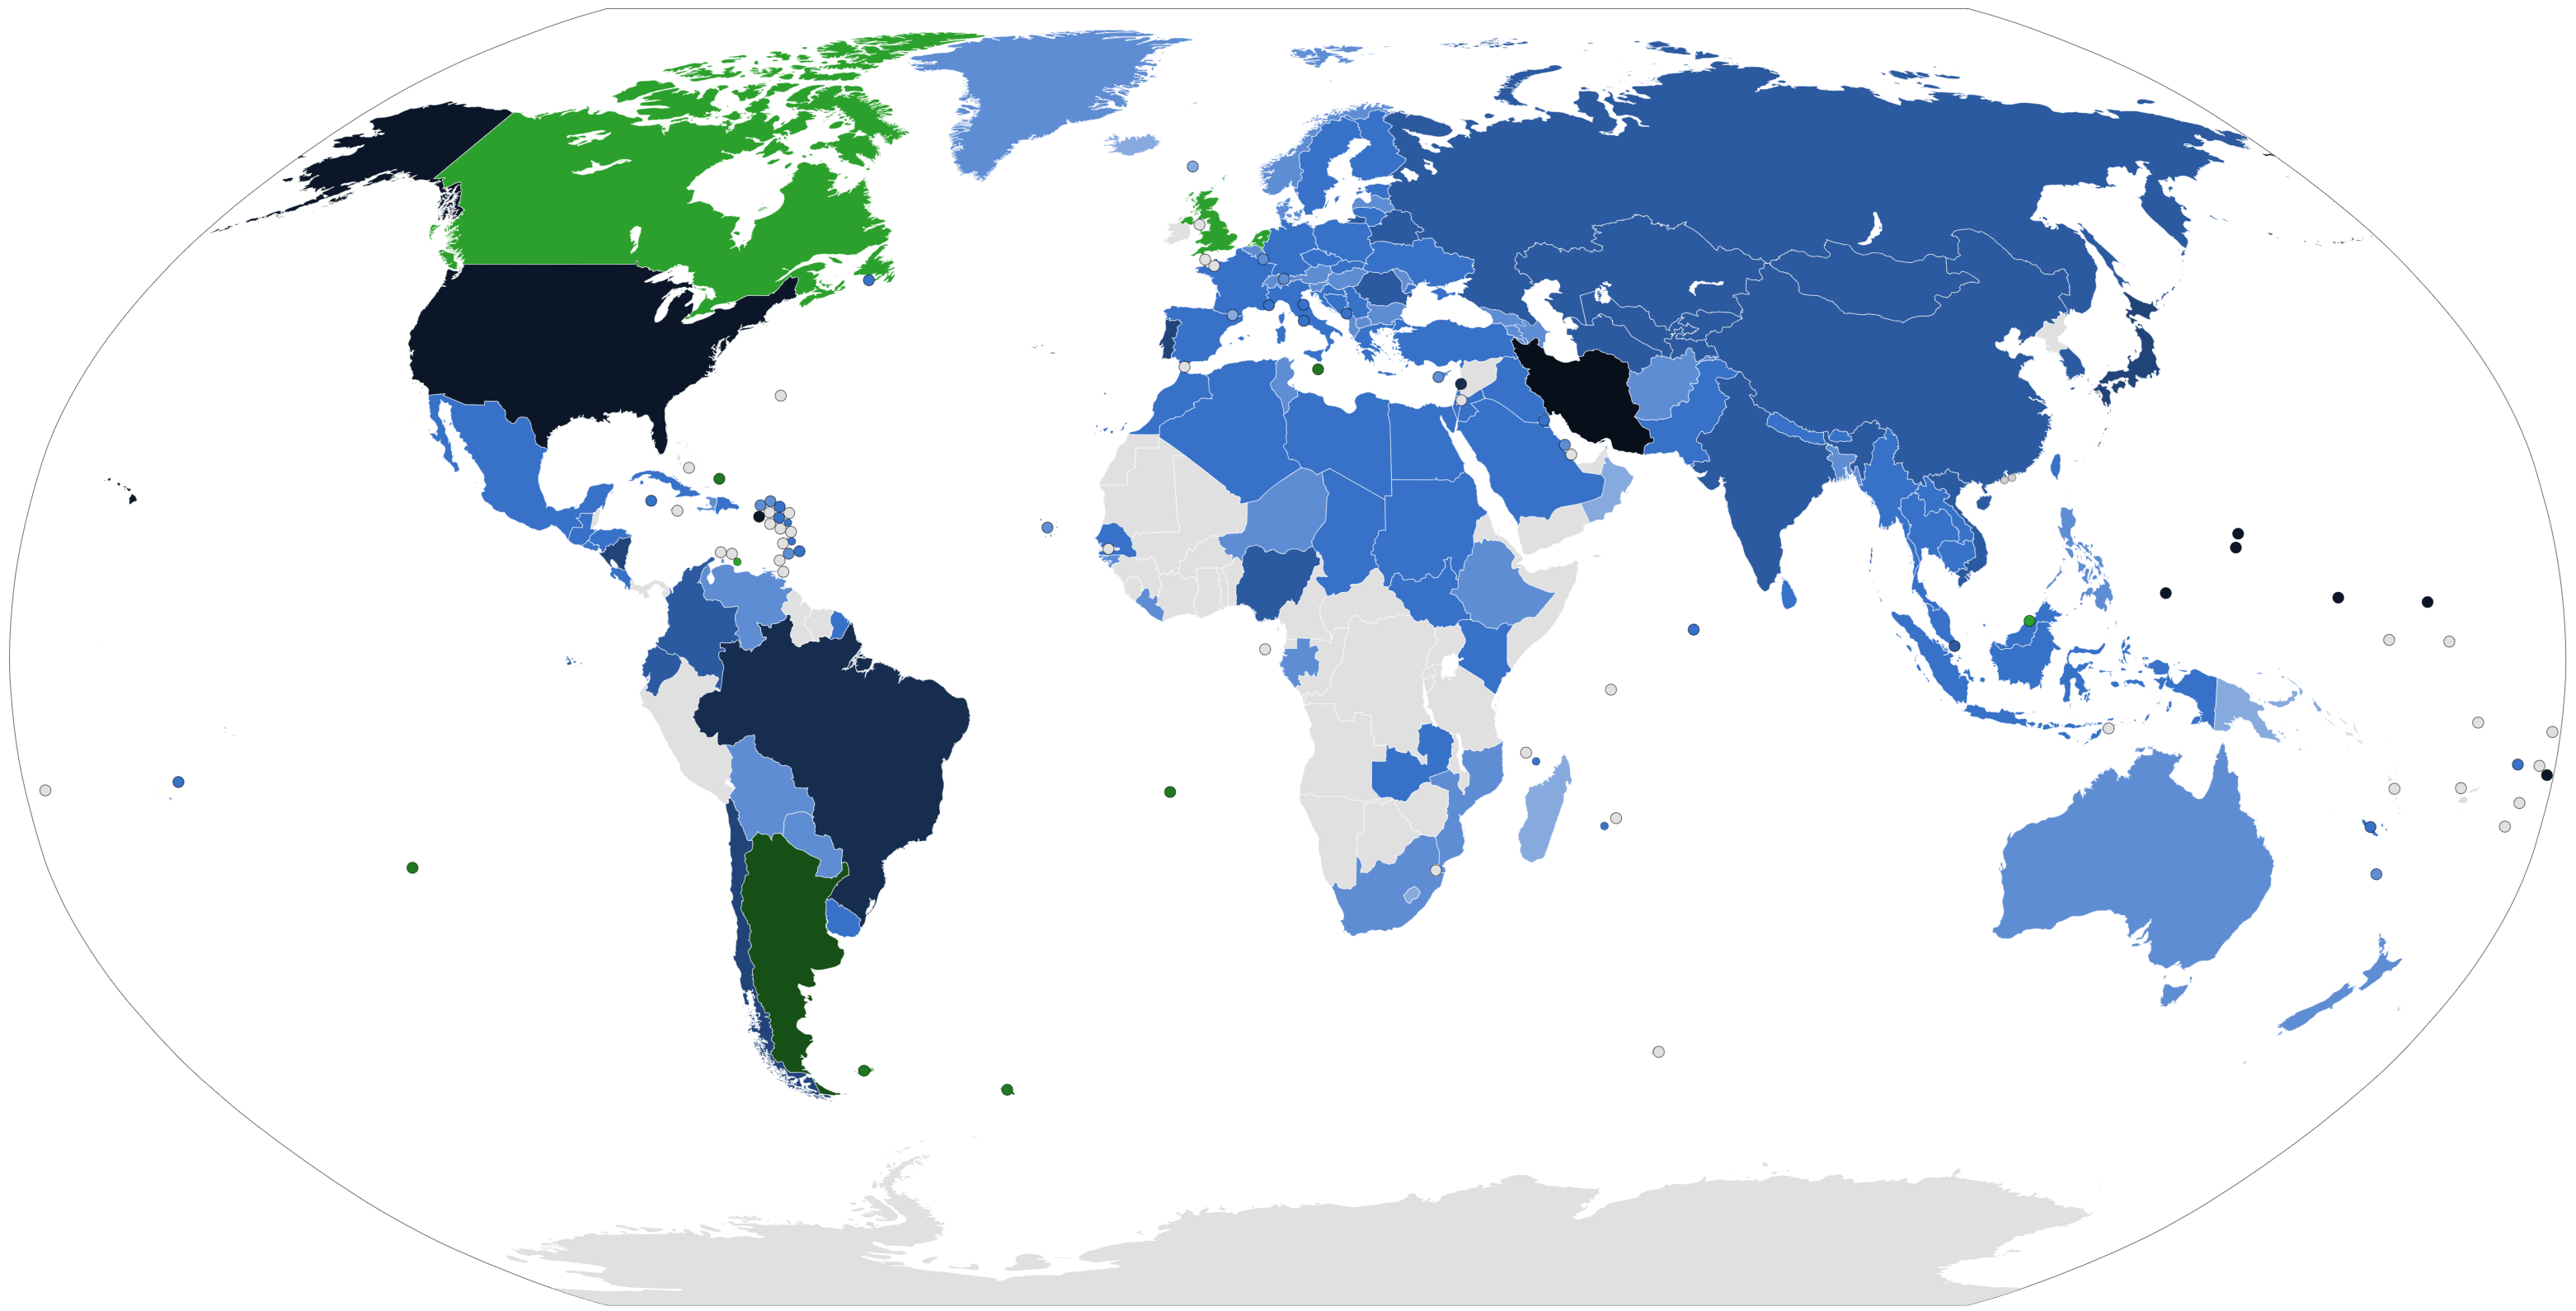
\includegraphics[width=1\textwidth]{PostalCodes}
	\caption[PostalCodes]{Postal codes by country with amount of digits ranging from three digits (lightblue) to eight digits (darkgreen) and no postal code system (gray)}
	\label{fig:postalcodes}
\end{figure}

Some downsides to using addresses and postal codes can be identified:

\begin{enumerate}
	\item Addresses can be ambiguous
	\item Addresses and postal codes can be imprecise
	\item Postal code systems are not uniform
	\item Some countries don't have postal code systems
\end{enumerate}

%%%%%%%%%%%%%%%%%%%%%%%%%%%%%%%%%%%%%%%%%%%%%%%%%%%%%%%%%%%%%%%%%%%%%%%%%%%%%%%%
% Literature review
%%%%%%%%%%%%%%%%%%%%%%%%%%%%%%%%%%%%%%%%%%%%%%%%%%%%%%%%%%%%%%%%%%%%%%%%%%%%%%%%
% - Storing location data
% - Querying location data
% - Intersecting
% - Research different countries
% - 3 words, gps, geospatial
%
\section{Literature Review}

What 3 words, a multi-award winning global addressing system, bases 3m x 3m squares, covering the planet, on a combination of three words.

Geospatial

Postal code

http://geoawesomeness.com/discrete-global-grid-system-dggs-new-reference-system/

\mynote{See if other people solved locations}

A polygon does not have such limitations.
In contrast, spatial datatypes would provide unique and precise location definition that is uniform and universal.

Many spatial database systems support a basic Geometry hierarchy of Points, Polygons, MultiPoint and MultiPolygon Classes, as described in the OGC~\cite{SFA} and ISO 19125~\cite{ISO-19125} standard, which are capable of mapping areas and points that are currently described by addresses and postal codes, and more. This answers the question whether postal codes can be abstracted to geospatial data, but has it retained its usefulness in the system?


A polygon could even describe the area of Belize City, which doesn't

- freedom of cutting amsterdam in half any way possible
- site of gps
- bermuda triangle

if a radius was assigned to the centroid of the shape that is formed by the boundaries of the street, neighbourhood, province or country. For example:

\begin{enumerate}[label*=\arabic*.]
	% Area, Polygon, Zipcode, Gps pair, Place, Collections
	\item Which location types matter for this project?
	% Polygons overlapping0
	\item Can a system be created that does not solely rely on postal codes?
				% 3 words, gps, geospatial,
	\item How can postal codes be abstracted to geospatial data while retaining the same usefulness in the system?
				% Show queries with box and star
	\item Which Database Management Systems (DBMS)s cover the location storage use cases for this project?
\end{enumerate}


\subsection{Location Related Scenarios}
The specific criteria to which the database geospatial functions must adhere are:

\begin{enumerate}
	\item the system must distinguish points inside and outside of a location.
	\item the system must detect whether a user travels from, or to, a point.
	\item the system must be able to handle overlapping locations.
	\item
	\item users should be able to select predefined locations from external sources.
\end{enumerate}





% The set of all possible lists of points, first and last point are equal
% and an area is a list of points in which the first and the last element are equal, thus closing the shape, for which there may be an equal shape in the form of a postal code area.
$A = \mathcal{P}(P)$

Finally, collections of these possibilities are allowed to describe the problematic "all churches in the Netherlands" example:

% A collection of points
$C_p \subseteq P$

and "all counties in which the majority voted Trump" example:

% A collection of areas
$C_a \subseteq A$.

This way a location could either be an area or a point, with which all possibilities are covered, except sets of these elements. As stated in Appendix \ref{appendix:pregame}, the definition of an area is precise, unambiguous and easy to use in compare in computer programs. A single point may match another single point if it’s the exact same point. A point may be sitting on top of a line or is contained within an area. The only other option is the negation of these statements. Because use cases for lines will be non-existent, points and areas are the proper candidates for spatial queries.

A taxi company director wants to be able to set price or define discounts from or to a certain location. They would like to define prices based only on departure locations, or only on destination locations, or both. For example: 'to Schiphol, a trip should cost \euro 10,-', or 'from van der Valk hotels, a trip should cost \euro 5,-', or 'from van der Valk hotels to Schiphol, the km price should be \euro 0,60'. In the current implementation, a record would be stored containing departure location, destination location and price for every combination, where locations were defined as zip codes. Instead, it would make sense to be able to reuse locations after they have been defined once.

%%%%%%%%%%%%%%%%%%%%%%%%%%%%%%%%%%%%%%%%%%%%%%%%%%%%%%%%%%%%%%%%%%%%%%%%%%%%%%%%
% Database Prerequisites
%%%%%%%%%%%%%%%%%%%%%%%%%%%%%%%%%%%%%%%%%%%%%%%%%%%%%%%%%%%%%%%%%%%%%%%%%%%%%%%%
% - Which Database Management Systems (DBMS) cover the location storage use
%   cases for this project?
%
\section{Database Prerequisites}
The database must be capable of determining whether a virtual perimeter contains a set of coordinates, more specifically, it must adhere to The Open Geospatial Consortium (OGC) Simple Feature Access ISO 19125-1 \cite{SFA} and ISO 19125-2 \cite{SFS}, including spatial data types, analysis functions, measurements and predicates for this requirement. The scenario presented in image \ref{fig:square} should be replicable.

\begin{figure}[htbp!]
	\centering
	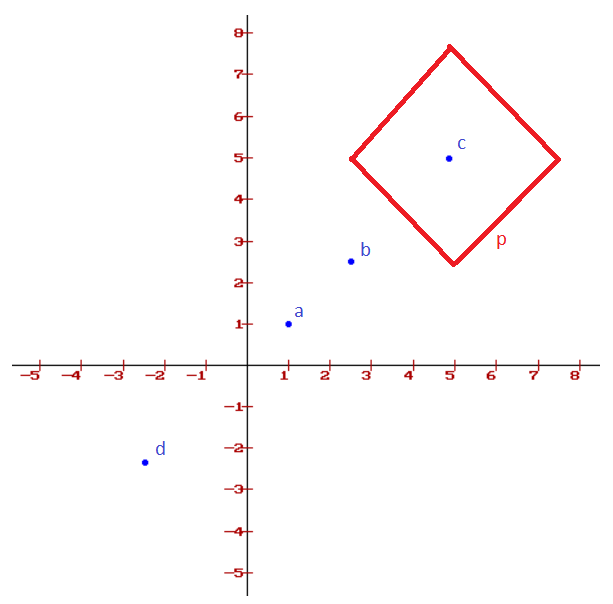
\includegraphics[width=.5\textwidth]{Square}
	\caption[Square]{Four Points, one Polygon p containing Point c.}
	\label{fig:square}
\end{figure}

\subsection{OpenGIS Compatible databases}
MYSQL’s innate integrity is a good reason to opt for a full MYSQL database setup. MariaDB is a fork of MYSQL that performs better according to benchmarks, however they don’t always translate to real life situations. It’s easy to migrate from MYSQL to MariaDB, so choosing MYSQL at first could be preferable as an instance of MYSQL is already used at TaxiID. PostgreSQL offers a spatial database extender for that is OpenGIS compliant called PostGIS that adds support for geographic objects and location queries.

All spatial data types inherit properties such as type and spatial reference identifier (SRID). For rigorous documentation, both PostGIS documentation \cite{PostGIS} and MYSQL documentation \cite{MySQL} could be consulted. When a generic geometry column, or point column is created, points can be inserted as shown in snippet \ref{lst:sql-insert-points} and \ref{lst:sql-insert-polygon}

\begin{multicols}{2}
	\begin{lstlisting}[caption={Insert four points}, label={lst:sql-insert-points}, belowskip=100pt]
	START TRANSACTION;
	SET @a = ST_GeomFromText('POINT(1 1)');
	INSERT INTO point (point) VALUES (@a);
	SET @b = ST_GeomFromText('POINT(2.5 2.5)');
	INSERT INTO point (point) VALUES (@b);
	SET @c = ST_GeomFromText('POINT(5 5)');
	INSERT INTO point (point) VALUES (@c);
	SET @d = ST_GeomFromText('POINT(-2.5 -2.5)');
	INSERT INTO point (point) VALUES (@a);
	# also insert @b, @c, and @d
	COMMIT;
\end{lstlisting}
	\begin{lstlisting}[caption={Insert polygon}, label={lst:sql-insert-polygon}, belowskip=0pt]
	START TRANSACTION;
	# First and last point must be the same
	SET @a = PolygonFromText('POLYGON((2.5 5,5 7.5,7.5 5,5 2.5,2.5 5))');
	INSERT INTO polygon (polygon) VALUES (@a);
	COMMIT;
\end{lstlisting}
\end{multicols}

It is evident that c is contained in p. To determine which points are contained in p, the function as seen in Snippet \mynote{Add ref to snippet} can be used, which returns the point with coordinates $[5, 5]$ as expected.

\begin{multicols}{2}
	\begin{lstlisting}[caption={Select points contained in polygon}, label={lst:sql-pts-in-poly}, belowskip=100pt]
	// All points contained in polygon
	SELECT ST_ASTEXT(POINT)
	FROM POINT
	WHERE
	ST_CONTAINS(
		(
			SELECT POLYGON
			FROM POLYGON
			WHERE id = 1
		),
		POINT
	)
\end{lstlisting}
	\begin{lstlisting}[caption={Select polygons containing point}, label={lst:sql-poly-has-pt}, belowskip=0pt]
	// All polygons containing point
	SELECT ST_ASTEXT(POLYGON)
	FROM POLYGON, POINT
	WHERE
		POINT.id = 3 AND ST_CONTAINS(
			POLYGON.polygon,
			POINT.point
		)
\end{lstlisting}
\end{multicols}

\subsection{OpenGIS Incompatible databases}
MongoDB doesn’t offer OpenGIS implementations but has geospatial query operators that may provide enough functionalities for current requirements \mynote{Add ref to Geospatial Query Operators — MongoDB Manual 3.6}. The argument for choosing one over the other depends on the vast differences between SQL and NoSQL, next to performance and extensiveness of geospatial features. The setup displayed in image \mynote{Add ref to image} is recreated in MongoDB using queries shown in snippet \mynote{Add ref to snippet}.

\begin{multicols}{2}
	\begin{lstlisting}[caption={Select points contained in polygon}, label={lst:sql-pts-in-poly}, belowskip=100pt]
	db.point.insertMany([
	{ shape: { type: "Point", coordinates: [1, 1] } },
	{ shape: { type: "Point", coordinates: [2.5, 2.5] } },
	{ shape: { type: "Point", coordinates: [5, 5] } },
	{ shape: { type: "Point", coordinates: [-2.5, -2.5] } },
	])

	db.polygon.insert({
	shape: {
	type: "Polygon",
	coordinates: [ [ [2.5, 5], [5, 7.5], [7.5, 5], [5, 2.5], [2.5, 5] ] ]
	}
	})

	db.point.createIndex({ 'shape': '2dsphere' })
	db.polygon.createIndex({ 'shape': '2dsphere' })
\end{lstlisting}
	\begin{lstlisting}[caption={Select points contained in polygon}, label={lst:sql-pts-in-poly}, belowskip=0pt]
	// All points contained in polygon
	var p = db.polygon.find({})

	db.point.find({
	shape: {
	$geoWithin: {
	$polygon: [
	[2.5, 5],
	[5, 7.5],
	[7.5, 5],
	[5, 2.5],
	[2.5, 5]
	]
	}
	}
	})

	// All polygons containing point
	var p = db.point.findOne({ coordinates: [5, 5] })

	db.polygon.find({
	shape: {
	$geoIntersects: {
	$geometry: {
	type: "Point",
	coordinates: [5, 5]
	}
	}
	}
	})
\end{lstlisting}
\end{multicols}

Next to database solutions for this requirement, services exist that are capable of geofencing. Although these services may not be free, and the added dependencies restrict extensibility.

%%%%%%%%%%%%%%%%%%%%%%%%%%%%%%%%%%%%%%%%%%%%%%%%%%%%%%%%%%%%%%%%%%%%%%%%%%%%%%%%
% Performance and Clustering Trade-offs
%%%%%%%%%%%%%%%%%%%%%%%%%%%%%%%%%%%%%%%%%%%%%%%%%%%%%%%%%%%%%%%%%%%%%%%%%%%%%%%%
%
\section{Performance and Clustering Trade-offs}
Agarwal and Rajan state that NoSQL take advantage of cheap memory and processing power, thereby handling the four V’s of big data more effectively,
but lack the robustness over SQL databases \mynote{Add reference to Agarwal and Rajan}. The report dives deeper into spatial queries and concludes that their tests suggest that MongoDB performs better by an average factor of 10, which increases exponentially as the data size increases, but lack many spatial functions that OpenGIS supports. Although improvements have been made \mynote{Add reference to Geospatial Performance Improvements in MongoDB 3.2,” MongoDB} after the cited paper Schmid et al. 2015 \mynote{Add ref to Stephan Schmid Eszter Galicz} was published. The team argues that clustering is much easier in MongoDB, which may be important in the future when the company grows. As the required functionalities exist in both SQL and NoSQL, it is beneficial to opt for MongoDB for its performance and alignment with the teams experience. Although if robustness is desired, or extra GIS functionalities required, SQL should be taken into consideration.
